% no \IEEEPARstart
% This demo file is intended to serve as a ``starter file''
% for IEEE Computer Society conference papers produced under \LaTeX\ using
% IEEEtran.cls version 1.8b and later.
% % You must have at least 2 lines in the paragraph with the drop letter
% % (should never be an issue)
% I wish you the best of success.

% \cite{Craford1992} reports something. 
% \cite{Muthu2002} ..
% \cite{LED_website}

% \hfill mds
 
% \hfill August 26, 2015

\subsection{Tetris}
Tetris is een videospel dat bedacht is door de wiskundige Alexey Pazhitnov \cite{Brzustowski_1992}. In het videospel moet je als speler alle vakjes van de lege rijen probeert in te vullen met willekeurige puzzelstukjes die uit de lucht vallen, totdat je één of meerdere hele rij(en) vol hebt. 
Zodra je één rij vol hebt, zal die rij verdwijnen en omgezet worden in een \(x\) aantal punten. Hetzelfde geldt voor: \textit{``double''} rijen, \textit{``triple''} rijen en een \textit{``TETRIS''} (vier rijen), hiervoor krijgt de speler uiteraard veel punten in ruil!
Het videospel heeft minimaal vier knopjes nodig om het spel te kunnen bedienen, hieronder is een lijstje te zien met welk knop wat doet:
\begin{enumerate}
    \item bovenste knop zorgt ervoor dat het object geroteerd kan worden;
    \item linker knop zorgt ervoor dat het object horizontaal naar links verplaatst;
    \item rechter knop zorgt ervoor dat het object horizontaal naar rechts verplaatst;
    \item onderste knop zorgt ervoor dat het object sneller naar beneden valt.
\end{enumerate}
Zoals al eerder verteld bevat Tetris allerlei verschillende puzzelstuk-vormen. Deze vormen worden ook wel Tetromino's genoemd \cite{Burgiel1997}. 
Er zijn zeven verschillende Tetromino's, namelijk:
\begin{enumerate}
    \item de ``Tee'', ook wel de T-vorm genoemd;
    \item de ``Left Kink'', ook wel de S-vorm genoemd;
    \item de ``Right Kink'', ook wel de Z-vorm genoemd;
    \item de ``Square'', ook wel O-vorm genoemd;
    \item de ``Left Elbow'', ook wel de L-vorm genoemd;
    \item de ``Right Elbow'', ook wel de J-vorm genoemd;
    \item de ``Bar'', ook wel de I-vorm genoemd.
\end{enumerate}
Zie figuur \ref{fig:Tetrominos} voor een betere verbeelding van hoe de Tetromino's er uit zien.
\begin{figure}[htbp]
    \centering
    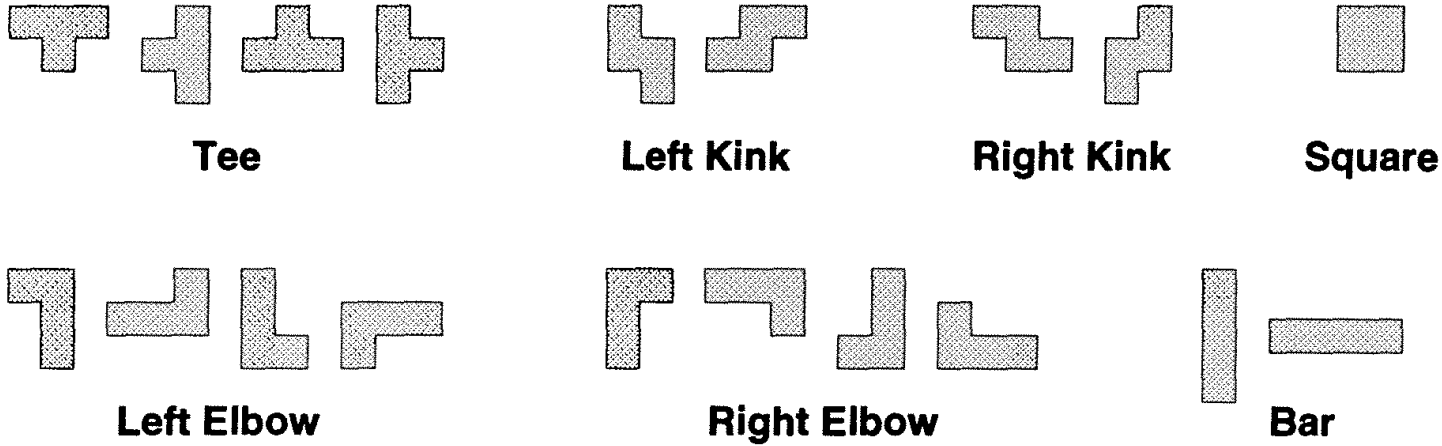
\includegraphics[width=0.5\textwidth]{Tetraminoes.png}
    \caption{Alle Tetromino's die in Tetris voor komen \cite{Burgiel1997}.}
    \label{fig:Tetrominos}
\end{figure}

Tetris heeft voor de rest nog een paar regels, namelijk:
\begin{enumerate}
    \item het is niet mogelijk om Tetromino's verder dan de rand van het spelgebied te verplaatsen;
    \item het is game-over als de Tetromino's de bovenkant van het scherm hebben bereikt;
    \item het is alleen mogelijk om rijen te verwijderen door één of meerdere rijen helemaal vol te hebben \cite{BREUKELAAR2004}. 
\end{enumerate}

\subsection{Microcontroller Unit}
Een microcontroller (afgekort: MCU of \(\mu C\)) moet je zien als een mini-computer drie draait op slechts één chip (single-chip). 
Deze chips worden ook wel IC's genoemd, dat afgekort ``Integrated Circuit'' betekent, dat is in het Nederlands vertaald: ``Geïntegreerde Schakeling''. 
In een IC zitten heel veel kleine elektrische componenten die op een ``semi-conducting material'' worden geplaatst \cite{ibrahim2006microcontroller}. 
Samen vormen deze kleine elektrische componenten een circuit in een zwarte behuizing op hele kleine schaal, vandaar dat het een geïntegreerde schakeling wordt genoemd. 
Naast de IC bestaat er ook een PIC, deze IC is programmeerbaar in programmeertalen C en C++ \cite{morton2005pic}.
Een normale IC is meestal voor één einddoel nodig en kun je niet zomaar een ander programma er op flashen. 
Een PIC kan dat wel, waarbij het wel mogelijk is om een programma erop te flashen. 
In dit project is er ook een PIC gebruikt, namelijk de ``PIC18F4520'' en op deze PIC staat het spel Tetris geprogrammeerd. 
Deze microcontroller (PIC18F4520) heeft in totaal 40 pins, zie figuur \ref{fig:PIC18F4520} voor de bijbehorende pin diagram.
\begin{figure}[htbp]
    \centering
    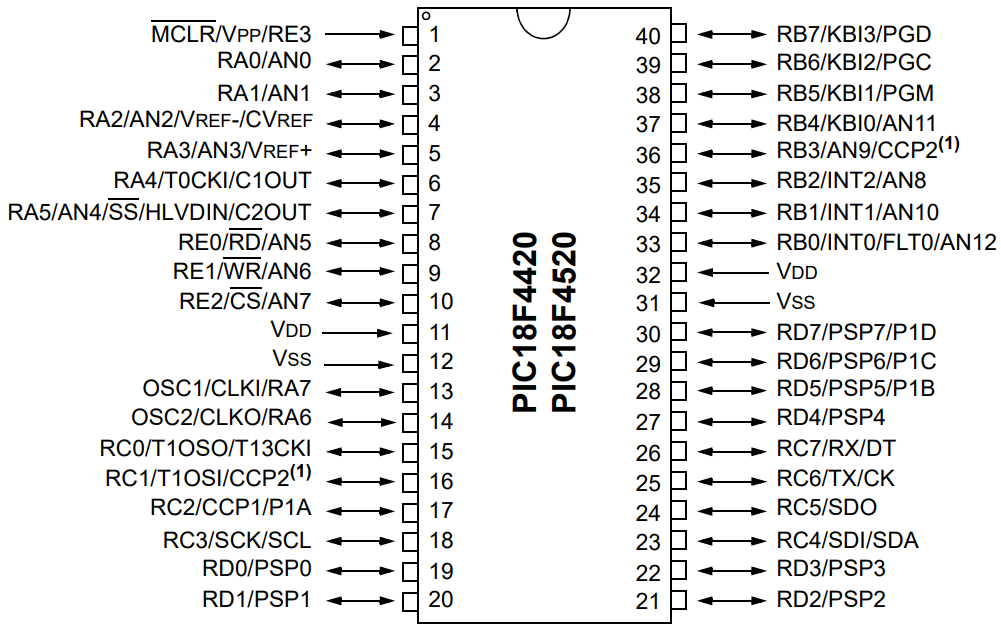
\includegraphics[width=0.5\textwidth]{PIC18F4520.png}
    \caption{Pin diagram van de 40-Pins PIC18F4520 \cite{PIC18F4520}.}
    \label{fig:PIC18F4520}
\end{figure}

Deze 40-pin PIC-microcontroller is gebruikt, omdat er twee 2x8-pin LED-matrixen, 3 pinnen voor de flash, 4x1-pin voor de knopjes en tenslotte nog 1x8-pin voor de secundaire IC. 
Daarnaast moeten er ook nog pinnen vrij blijven voor de \(V_{DD}\) (+) en \(V_{SS}\) (-) aansluitingen en dat zijn er vier in totaal, dus er worden in totaal minimaal 35 pinnen gebruikt \cite{PIC18F4520}.

Bij dit project horen natuurlijk ook deelvragen en een onderzoeksvraag. Hieronder zie je een lijst met de deelvragen, namelijk: 
\begin{enumerate}
    \item Wat is de definitie van een blokschema? Ontwerp een blokschema voor het spelletje PICtris;
    \item Welke soorten LED's bestaan er? Leg uit welke uitvoeringen en maatvoeringen er zijn;
    \item Wat zijn de elektrische eigenschappen van een aantal kleuren LED's?
    \item Wat zijn de elektrische gevolgen van deze eigenschappen?
    \item Ontwerp een eenvoudige schakeling waarin een LED is aangesloten op een spanningsbron van 5V. Wat zijn de elektrische gevolgen van deze basisschakeling? 
    \item Wat zijn pull-up en pull-down weerstanden en waar worden ze voor gebruikt? Maak een ontwerp waarbij er een schakelaar gebruikt wordt op een \(\mu C\) die altijd een gedefinieerde toestand heeft.
\end{enumerate}

De onderzoeksvraag die in dit artikel wordt beantwoord is:
\textit{``Hoe kan de PIC18F4520 microcontroller gebruikt worden om een Tetris gameboy te bouwen met de verkregen componenten en middelen, waaronder de Tetris code?''}